\chapter{Synthesis}
\label{chap:synthesis}

% TODO
This chapter describes the problem statement, its definition, and the approaches
that were studied in order to try to solve it. The first one, described in
section ???, is based on a component-based constraint solving approach presented
by~\citeauthor{Jha:oracle:2010} when applied to ... and further explored in
their ogis paper \cite{Jha:oracle:2010}...

% TODO
\todo{We are working in the context of OutSystems...}{concept of readability,
  usability, etc. That the programs are outsystems expressions, etc.}

The programs we are interested in are expressions in the OutSystems language
\footnote{\url{https://success.outsystems.com/Documentation/11/Reference/OutSystems_Language/Logic/Expressions}}.
In the context of this work, we can think of OutSystems expressions as a simple
functional language of operands and operators that compose themselves to create
pure, stateless, tree-like programs. This means that OutSystems expressions do
not have side-effects, like printing to the screen, or writing to a database,
and do not permit any variables or loops. They do, however, have conditional
expressions in the form of ``if'' statements. The library of builtin expressions
includes functions that manipulate builtin data types such a text strings,
numbers, or dates.

% TODO Example of an outsystems expression
\todo{Listing x includes examples of outsystems expressions. These do y and z.}{}

% TODO Explain how it fits in the context of service studio and how it interacts
% with other features (like being able to manipulate structures and lists).
This language of expressions fits on ...

We do not have access to actual input-output data, which swayed the kind of
approaches we took in order to solve this problem. For example, we could not
use approaches that applied inductive reasoning to a corpus of pre-existing
input-output examples in order to find some common patterns 

% of expression usage.

% TODO FIXME
We had access to 10239847012983 OutSystems expressions, with sizes ranging from
x to y, and manipulating data types such as z and w. The most used functions
were ... and typical programming patterns included ...

\section{Problem Statement}
\label{sec:problem-statement}

In our context, we are working in a \gls{pbe} setting, so we are interested in
synthesizing an OutSystems expression from a set of input-output examples
$\{(I_i, o_i)\}_i$.

Because OutSystems expressions are composed of self-contained pure functions,
this synthesis problem fits nicely in the component-based synthesis paradigm.
Therefore assume we are given a \textit{library} of base components $F$ that the
synthesizer can use in order to make the programs. These components will be the
builtin functions drawn from the OutSystems library. Each component can take a
finite number of inputs and return exactly one output. The allowed types for the
inputs and the output are \todo{text strings and integers}{expand?}.

More formally, a component $f \in F$ is represented by an expression
$\phi{}_f$ that specifies how its input parameters $P_f$ relate to its
return value $r_f$.

% TODO Add an example of one or two components and their possible specs

% FIXME fix the literals
OutSystems expressions can also have constant literals, like
\lstinline{"string"}, or \lstinline{0}. These can either be given by the user as
extra information, or figured out automatically by the synthesizer.

If we ignore well-typedness, an OutSystems expression is a tree-like program
whose form can be succintly described using a \gls{cfg}:

\begin{center}
  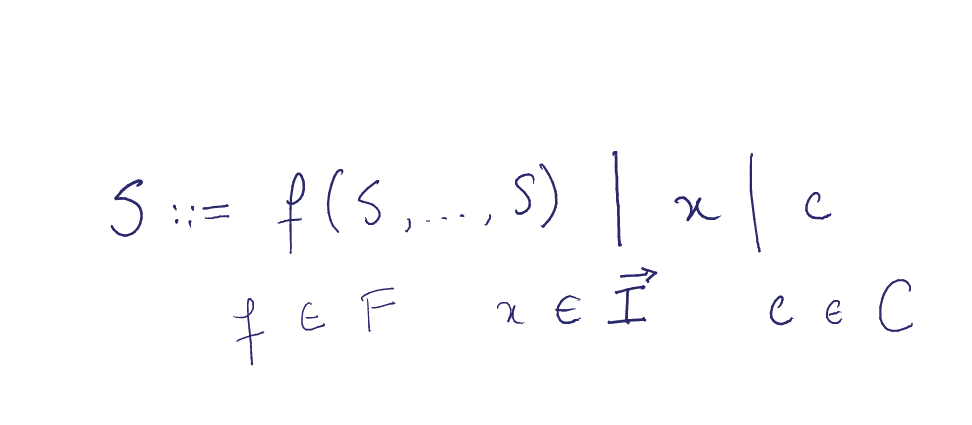
\includegraphics[width=0.7\textwidth]{assets/cfg-expressions.png}
\end{center}

% TODO Show grammar here.

where $I$ denotes the set of inputs from a given input-output example, and
$C$ is the set of constant literals in the OutSystems language.


\section{A First Approach}
\label{sec:first-approach}

It is useful to reason about OutSystems expressions in another representation,
called \gls{ssa}. A program in \gls{ssa} form is a line program with variables
where every variable is assigned exactly once and defined before its use. For
example, the program from Figure ??? could be written in \gls{ssa} form in the
following manner:

% TODO Show program in SSA form

This program format can be described succintly with the following \gls{cfg}:

% TODO Show cfg for programs in SSA form
$S ::= y \leftarrow c | y \leftarrow f(x_1, ..., x_n) | S;S$

The non-terminal $S$ represents a line in the program. A line is an assignment
of a variable to a constant literal $c$ or to the return value of a component
$f$ on inputs $x_1, ..., x_n$. Thus, the structure of a program in \gls{ssa}
form is a sequence of assignments.

The approach described in this section is based on
\citeauthor{Jha:oracle:2010}'s program encoding. The idea is to encode the
program space in a formula that is then constrained further in order to encode
only those programs that satisfy the input-output examples. A solution to this
formula can then be decoded back yielding a program that satisfies the set of
examples.

The synthesizer follows the \gls{ogis} model, described in
Section~\ref{sec:ogis}. It has a learner part and an oracle part, which will
call here the \textit{enumerator} and the \textit{solver}, respectively.

The enumerator receives the input-output examples as input, and is parameterized
by the library of base components. The enumerator is responsible for drawing a
subset of components from the library. It then passes these components to the
solver, along with the input-output examples, and queries whether there is any
program made only of those components that satisfies the examples. There is an
additional restriction that the program must use each of the components exactly
once.

% TODO Explain how the enumerator draws the components

The solver works by encoding the query into an \gls{smt} formula, and uses an
automated SMT solver to check for satisfiability. The SMT solver might or might
not be able to solve the formula. If the formula is satisfiable, the solver
responds to the enumerator with SAT and a solution to that formula. If not, it
responds UNSAT or UNKNOWN, depending on whether the formula is unsatisfiable or
the SMT solver could not verify its satisfiability, respectively.

The procedure finishes when enumerator receives SAT from the solver: the
enumerator decodes the solution to the formula into an actual program, and
outputs it.

% TODO Insert here a listing of the program

\subsection{Encoding}
\label{sec:encoding}

\todo{TODO}{}

``Each connection is encoded using an integer-valued location variable.''

\(N = |I| + |C|\)

Formula for syntactically well-formed programs:

\begin{align*}
  \phi{}_{wfp} &= \bigwedge_{f \in F}\bigwedge_{p \in P_f} (1 \leq l_p \leq l_f) \\
  &\wedge \bigwedge_{f \in F} (N + 1 \leq l_f \leq N + |F|) \\
  &\wedge \bigwedge_{\substack{r_1, r_2 \in R\\ r_1 \not\equiv r_2}} (l_{r_1} \neq l_{r_2})
   \wedge \bigwedge_{\substack{r_1, r_2 \in R\\ r_1 \not\equiv r_2}} (l_{r_1} \neq l_{r_2}) \\
  &\wedge \bigwedge_{p \in P}\bigwedge_{\substack{x \in I \cup C \cup R \cup \{o\} \\ kind(p) \neq kind(x)}} (l_p \neq l_x)
   \wedge \bigwedge_{\substack{r \in R \\ kind(r) \neq kind(o)}} (l_r \neq l_o)
\end{align*}

Semantics:

\begin{align*}
  \phi{}_{spec} &= \bigwedge_{f \in F} \phi{}_f (I_f, o_f) \\
  \phi{}_{flow} &= \bigwedge_{p \in P}\bigwedge_{\substack{x \in I \cup C \cup R \\ kind(p) \neq kind(x)}} (l_p = l_x \implies p = x)
\end{align*}

All inputs used:

\[ \phi{}_{in} = \bigwedge_{i \in I}\bigvee_{p \in P}(l_i = l_p) \]

All outputs used:

\begin{align*}
  \phi{}_{out} &= \bigwedge_{f \in F}\bigvee_{p \in P - P_f}(l_f = l_p) \\
               &\vee \bigwedge_{f \in F} (l_f = l_o)
\end{align*}

Constrain the length of string constants:

\[
  \phi{}_{len} = \bigwedge_{\substack{c \in C \\ kind(c) = string}} len(c) \leq 5
\]

Extra:

\[ \phi{}_{extra} = \phi{}_{in} \wedge \phi{}_{out} \wedge \phi{}_{len} \]

Formula for a single run of a program:

\begin{align*}
  \phi{}_{prog} = \exists P,R\ldotp (\phi{}_{wfp} \wedge \phi{}_{spec} \wedge
  \phi{}_{flow} \wedge \phi{}_{extra})
\end{align*}

The full formula:

\[
  \Phi{} = \exists L\ldotp \bigwedge_{(I, o) \in E}\phi{}_{prog}
\]

We could also try:

\[
  \Phi{} = \exists L\ldotp \forall (I, o) \in E \ldotp \phi{}_{prog}
\]



% TODO Concrete example of the encoding of a program